\section{Forsøgte metoder}
Hvis man ser på en række vesikler, er det tydeligt at de ikke er ens. De har forskellig størrelse, både i kantens tykkelse og i diameteren. To eksempler på vesikler er vist i figur \ref{fig:premethod_ves1}, hvor det fremgår at de begge er relativt cirkulære. At vesiklerne er meget forskellige fremgår også tydeligt af figuren. Selvom begge har nogenlunde samme farve kant har vesiklen til venstre et meget lyst indre, hvor vesiklen til højre er meget mørkere. 

I introduktionen talte vi om hvor meget støj der var omkring alle vesiklerne, og hvordan det derfor var svært at se overgangen i kanterne. Det er derfor klart at der skal være en form for udglatning af billedet for at undertrykke støjen, og om muligt også et filter der kan fremhæve de interessante værdier.

\begin{figure}[H]
	\begin{minipage}[b]{0.5\linewidth}
		\centering
		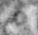
\includegraphics[scale=5]{files/premethod/img/ves1.png}
	\end{minipage}
	\hspace{0.5cm}
	\begin{minipage}[b]{0.5\linewidth}
		\centering
		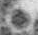
\includegraphics[scale=5]{files/premethod/img/ves2.png}
	\end{minipage}
	\caption{To udsnit af en enkelt vesikel. Begge vesikler er relativt cirkulære.\label{fig:premethod_ves1}}
\end{figure}

\subsection{Metoderne}	
At vesiklerne har fællestræk men alligevel er så forskellige, antyder at en enkelt metode ikke vil finde alle vesiklerne, og at vi i stedet skal kombinere flere metoder der tilsammen kan finde alle typer af vesikler.

Det faktum at nogen af vesiklerne er relativt cirkulære, giver os ideen at detektere cirkler i billedet. Til dette benytter vi os af Hough cirkeldetektion. Metoden er forklaret nærmere i afsnit \ref{premethod_hough}, men for at metoden kan fungere, skal billedet behandles først. Her benytter vi et Gauss filter der udglatter billedet før et sobel filter finder retninger i billedet som en kantdetektor bruger til at finde hvor der er kanter i billedet. Hver af disse funktioner er forklaret nærmere nedenfor, og vi vil til slut evaluere på resultatet.

Vi vil benytte celleudsnittet i figur \ref{fig:premethod_celle} til at finde vesikler i. Billedet er godt da det både indeholder støj, vesikler og kant på cellen hele vejen rundt.

\begin{figure}[H]
	\centering
	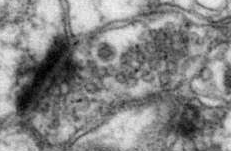
\includegraphics[scale=2.5]{files/premethod/img/celle1.png}
	\caption{Celleudsnit fra originalbilledet.\label{fig:premethod_celle}}
\end{figure}

\subsubsection{Gaussisk blur}
Et gaussisk blur, eller gaussisk udglatning, er i virkeligheden et lavpasfilter da funktionen i virkeligheden reducerer billedets højfrekvens værdier. Filteret bliver typisk brugt til at reducere billedstøj og udglatte områder. 

\begin{figure}[H]
	\begin{minipage}[b]{0.5\linewidth}
		\centering
		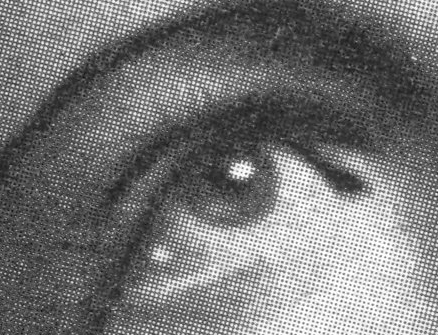
\includegraphics[scale=1.5]{files/premethod/img/gauss_pre.png}
	\end{minipage}
	\hspace{0.5cm}
	\begin{minipage}[b]{0.5\linewidth}
		\centering
		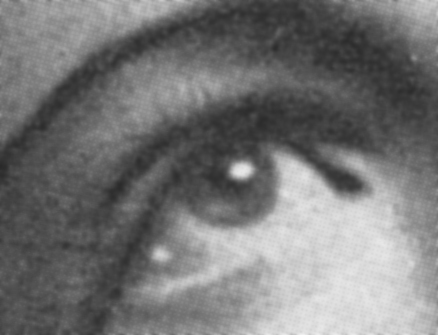
\includegraphics[scale=1.5]{files/premethod/img/gauss_post.png}
	\end{minipage}
	\caption{Billede før og efter en Gauss udglatning.\label{fig:premethod_gauss}}
\end{figure}

I figur \ref{fig:premethod_gauss} ses to billeder hvor det første er originalbilledet og det andet er billedet der er blevet behandlet med gaussfilter. Resultatet er tydeligt, billedet er glattere og med mindre støj. Dette er hvad vi er interesseret i, for at fjerne noget af støjen omkring vesiklerne, samtidig med at glatte kanten lidt ud. I to dimmensioner er ligningen for en gaussisk funktion givet ved ligningen
\begin{align}
	G(x,y) = \frac{1}{2\pi\sigma^2}e^{-\frac{x^2+y^2}{2\sigma^2}}\label{ali:premethod_gaussG}
\end{align}
hvor x er distancen fra origo på den horisontale akse, y er distancen fra origo på den vertikale akse og $\sigma$ er standard afvigelsen af den gaussike fordeling. Når man omtaler størrelsen på den gaussiske kerne er det størrelsen på dimensionen for $G$ der bygges. Ser vi på (\ref{ali:premethod_gaussG}) så er det kun eksponentialdelen der ændrer sig når x og y ændres. Vi ser så at et større x og y får eksponentialdelen til at gå mod 0. At hæve $\sigma$ værdien vil betyde at eksponentialdelen går langsommere mod 0. Der er ikke nogen grund til at lave en matrix med den gaussiske fordeling større end dens indgange har værdier på tal større end 0. Da vi er ude efter at udglatte billeder med vesikler på størrelse med ca. 20x20 pixels, ønsker vi at bygge et gaussisk fordelingsmatrix en smule større end dette, f.eks. på 30x30 pixels. Vi vælger derfor et $\sigma$ der gør at $G(30,30) > 0$. I figur \ref{fig:premethod_gauss_table} ses en oversigt over $G(30,30)$ med $\sigma$ værdier varierende fra 5 til 15. Det ses at $\sigma$ værdier på 5-10 er meget lave, og vi vælger derfor $\sigma$ til at have værdien 15.  
 
\begin{figure}[H]
	\centering
	\begin{tabular}{l | l}
			\textbf{$\sigma$} & $G(30,30)$\\
			\hline
			$5$ & $1.476654096\cdot10^{-18}$\\
			$6$ & $6.139819206\cdot10^{-14}$\\
			$7$ & $3.425994239\cdot10^{-11}$\\
			$8$ & $1.942558050\cdot10^{-9}$\\
			$9$ & $2.936573462\cdot10^{-8}$\\
			$10$ & $1.964128034\cdot10^{-7}$\\
			$11$ & $7.740076025\cdot10^{-7}$\\
			$12$ & $0.000002133620264$\\
			$13$ & $0.000004582712125$\\
			$14$ & $0.000008229144803$\\
			$15$ & $0.00001295566429$
	\end{tabular}
	\caption{Tabel over gaussisk fordeling i pixel 30,30 efter forskellige $\sigma$ værdier.\label{fig:premethod_gauss_table}}
\end{figure}

I figur \ref{fig:premethod_GaussCelle} ses vores cellebillede fra figur \ref{fig:premethod_celle} der er blevet behandlet med et gaussfilter. Det er tydeligt at billedet er blevet udglattet, men det er samtidig også blevet sværere at se overgangen mellem vesiklerne. Dette er ikke et positivt resultat og vi forkaster funktionen.

\begin{figure}[H]
	\centering
	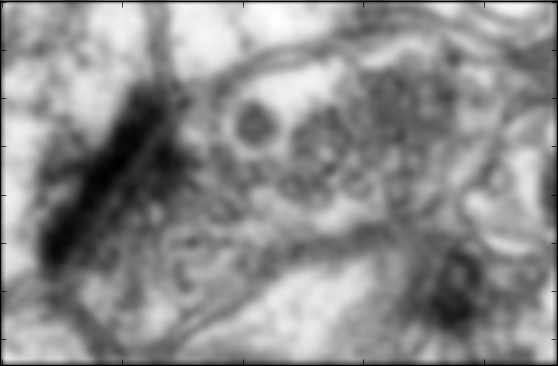
\includegraphics[scale=0.8]{files/premethod/img/gausscell.png}
	\caption{Celleudsnit behandlet med et gaussfilter og $\sigma$ værdi på 15.\label{fig:premethod_GaussCelle}}
\end{figure}


\subsubsection{Sobel filter og kantdetektion}
I billedbehandling benyttes Sobel operatoren især i kant detektion. Operatoren udregner gradienten for hvert punkt i billedet. Gradienten i et billede er en retningsændring i intensitet eller farve i et billede. Det resulterende billede indeholder så retningen i den størst mulige ændring fra lys til mørk. Jo lysere en pixel er, jo større sandsynlighed er der for at den er en del af en kant. Et eksempel på et billede der er blevet behandlet med et sobelfilter ses i figur \ref{fig:premethod_sobelres}

\begin{figure}[H]
	\begin{minipage}[b]{0.5\linewidth}
		\centering
		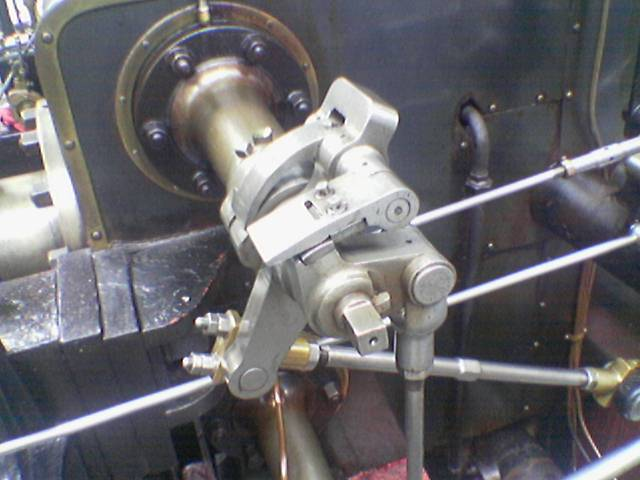
\includegraphics[scale=0.25]{files/premethod/img/sobel1.PNG}
	\end{minipage}
	\hspace{0.5cm}
	\begin{minipage}[b]{0.5\linewidth}
		\centering
		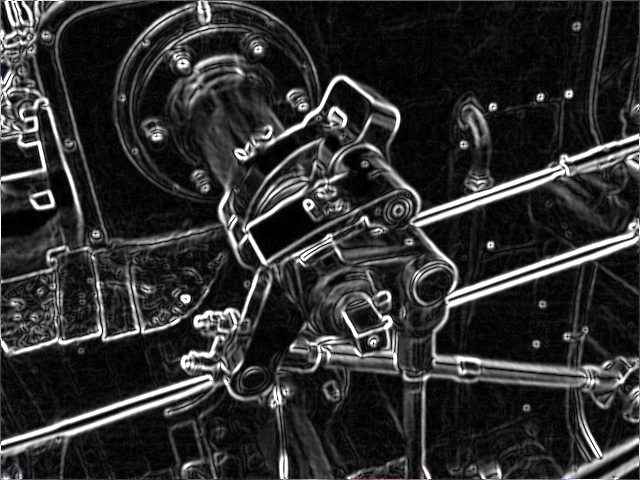
\includegraphics[scale=0.25]{files/premethod/img/sobel2.PNG}
	\end{minipage}
	\caption{Originalbilledet til venstre, og behandlet med et sobel filter til højre.\label{fig:premethod_sobelres}}
\end{figure}

At beregne et billede der er blevet behandlet med et sobelfilter er ikke særlig dyrt i forhold til udregninger, da operatoren baserer sig på at folde billedet med et lille separabel integer filter først i horisontal og så i vertikal retning. Hver af filtrene repræsenterer sin egen retning, så $G_x$ er defineret som hvordan gradienten ændrer sig i højregående retning, og $G_y$ er hvordan gradienten ændrer sig i nedadgående retning. $G_x$ og $G_y$ defineret i  (\ref{ali:premethod_sobelG}), hvor $I$ repræsenterer originalbilledet der foldes med, og $*$ operatoren betyder foldning.

\begin{align}
	G_y = \begin{bmatrix}
		-1 & -2 & -1\\
		0 & 0 & 0\\
		1 & 2 & 1
	\end{bmatrix} * I
	&&
	G_x = \begin{bmatrix}
		-1 & 0 & 1\\
		-2 & 0 & 2\\
		-1 & 0 & 1
	\end{bmatrix} * I
	\label{ali:premethod_sobelG}
\end{align} 

Det resulterende sobel billedes fås ved formlen 
\begin{align}
	G = \sqrt{G_x^2 + G_y^2}
\end{align}

På ethvert tidspunkt kan vi så finde retningen som kanten har i enhver pixel ved 
\begin{align}
	\Theta = \arctan\left(\frac{G_y}{G_x}\right)
	\label{ali:premethod_sobelTheta}
\end{align}
hvor $\Theta$ er 0 for en vertikal kant med mørkt på den venstre side. Vi skal bruge disse formler senere når vi ser på Hough cirkel detektionen der benytter sig af sobelfilteret når det skal finde kanter. 

\begin{figure}[H]
	\centering
	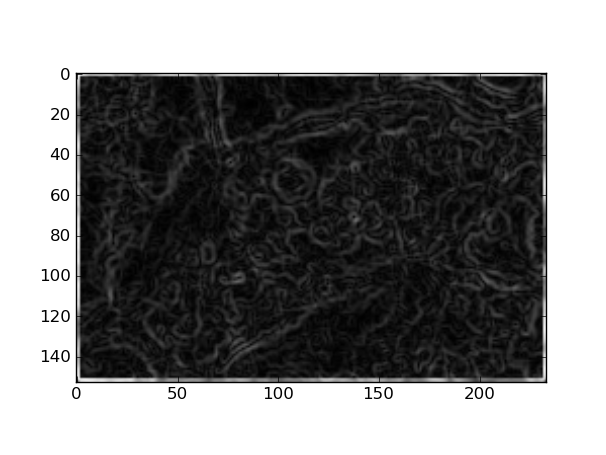
\includegraphics[scale=0.8]{files/premethod/img/sobel.png}
	\caption{Originalbilledet foldet med et sobelfilter.\label{fig:premethod_sobel}}
\end{figure}

Det resulterende sobel billede vil kun fremstå med værdi større end 0 i de pixels man med stor tiltro mener er en kant. Originalbilledet fra figur \ref{fig:premethod_celle} foldet med sobelfilteret ses i figur \ref{fig:premethod_sobel}. 

Dette er ikke noget særlig godt billede da kanterne omkring vesiklerne ikke fremstår tydeligere end støjen. Vi havde håbet på en kant der fremstod klart lysere end resten så vi med en tærskelværdi kunne isolere disse kanter. Vi har alligevel påført en tærskelværdi på 40 på billedet, og resultatet ses i figur \ref{fig:premethod_sobel}.

\begin{figure}[H]
	\centering
	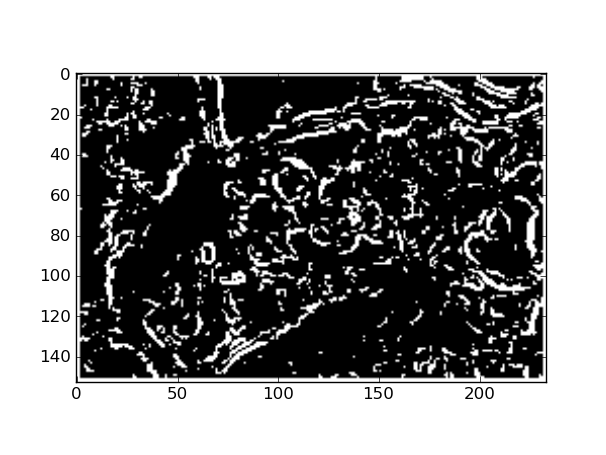
\includegraphics[scale=0.8]{files/premethod/img/edgemap.png}
	\caption{Sobelfilteret fra figur \ref{fig:premethod_sobel} med en tærskelværdi på 40.\label{fig:premethod_edgemap}}
\end{figure}

Her er det stadig tydeligt at der er meget andet støj end de vesikler der skal detekteres. Hvis vi ændrer tærskelværdien vil noget af støjen forsvinde, men det samme vil vesiklerne selv, så dette er ikke en mulighed.

\subsubsection{Hough detektion}\label{premethod_hough}
I de tidligere afsnit har vi vist hvordan vi har udglattet billedet, fundet kanter og retninger i hver af disse kanter. Disse resultater vil vi nu benytte til at finde cirklernes centrum. I (\ref{ali:premethod_sobelG}) har vi fundet $G_x$ og $G_y$ som jo var gradienterne i horisontal og vertikal retning. Vi fandt også $\theta$ i (\ref{ali:premethod_sobelTheta}), der er vinklen på en kant i den givne pixel. Vi har i vores observationer af vesiklerne også fundet ud af at de kan variere i størrelse fra 15x15 pixel, og op omkring 30x30 pixels.

Ideen er så at tage hver pixel der har en værdi større end 0 i kantbilledet efter tærskelværdien, altså hver pixel der menes at ligge på en kant, og tegne en linje ud fra denne. Linjen tegnet i en nyt canvas på samme størrelse som det originale billede, og hver pixel linjen går igennem, ligges en farveværdi oveni. Hvis hver linje så har en farveværdi på 10, og der så er 20 linjer der alle går igennem samme punkt, vil dette punkt få en farveværdi på 200. Man kan så tage en tærskelværdi på dette billede, og tilbage vil være de punkter der gerne skulle være centrum i en cirkel. 

Da vi ved at en vesikel har radius på min og maks hhv. 7.5 og 15, og vi kender $\theta$ kan vi nemt udregne ligningen for linjen der står vinkelret på punktet [i,j] (der menes at være et punkt på en kant) og har minimumsradius på 7.5 og maksimumsradius på 15. En af disse linjer ses i figur \ref{fig:premethod_houghLines}. 

\begin{figure}[H]
	\centering
	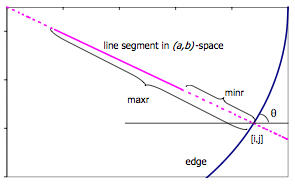
\includegraphics[scale=1]{files/premethod/img/hough_lines.png}
	\caption{Linje tegnet ud fra pixel [i,j] der menes at ligge på en kant.\label{fig:premethod_houghLines}}
\end{figure}

I figur \ref{fig:premethod_houghres} ses 4 billeder. Den første er bare en normal cirkel vi ønskes at detektere. I det andet billede er så tegnet nogle af de linjer der går igennem et punkt på kanten af cirklen samt centrum af cirklen. Her har vi ikke bekymret os om minimumsradius, ligesom vi kun har tegnet 6 af linjerne. I det tredje billede ses de samme linjer bare tegnet i det nye canvas. I det fjerde og sidste billede er der så taget en tærskelværdi på det resulterende canvas, og centrum der dermed fundet.

\begin{figure}[H]
	\begin{minipage}[b]{0.5\linewidth}
		\centering
		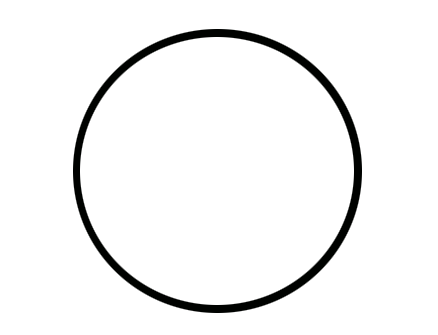
\includegraphics[scale=1.5]{files/premethod/img/dirmap1.png}
	\end{minipage}
	\hspace{0.5cm}
	\begin{minipage}[b]{0.5\linewidth}
		\centering
		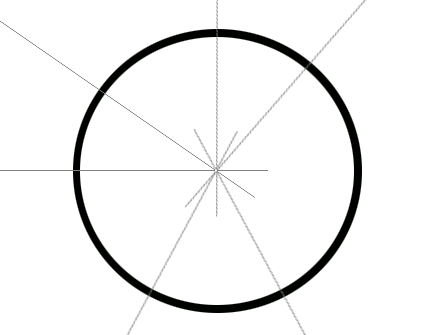
\includegraphics[scale=1.5]{files/premethod/img/dirmap2.png}
	\end{minipage}\\\\
	\begin{minipage}[b]{0.5\linewidth}
		\centering
		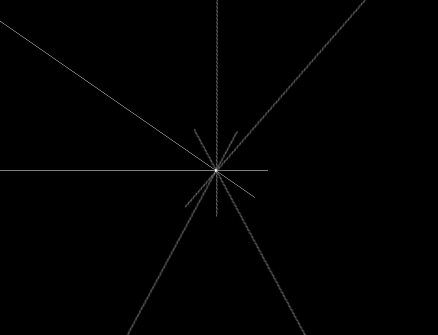
\includegraphics[scale=1.5]{files/premethod/img/dirmap3.png}
	\end{minipage}
	\hspace{0.5cm}
	\begin{minipage}[b]{0.5\linewidth}
		\centering
		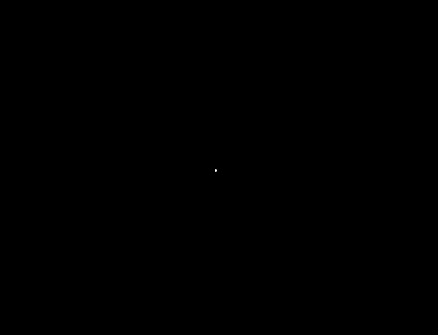
\includegraphics[scale=1.5]{files/premethod/img/dirmap4.png}
	\end{minipage}
	\caption{\textbf{Øverst venstre:} Originale billede. \textbf{Øverst højre:} Cirkel med nogen af linjerne tegnet. \textbf{Nederst venstre:} Det resulterende billede med nogen af linjerne tegner. \textbf{Nedest højre:} Resultat efter tærskelværdi.\label{fig:premethod_houghres}}
\end{figure}

Vi forsøger os så med vores sobel behandlede billede fra figur \ref{fig:premethod_edgemap}. Vi tegner linjer ud fra hver af disse punkter med minimumsradius på 7.5 og maksimumsradius på 15, og det resulterende billede ses i figur \ref{fig:premethod_houghCellLines}. 

\begin{figure}[H]
	\centering
	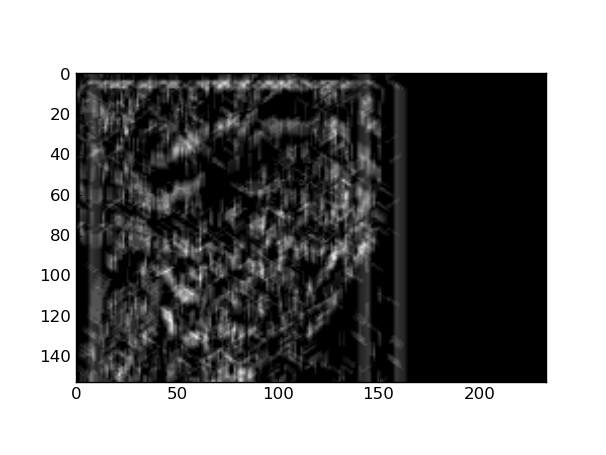
\includegraphics[scale=0.8]{files/premethod/img/houghCell.png}
	\caption{Houghlinjer tegnet ud fra sobelbilledets kanter.\label{fig:premethod_houghCellLines}}
\end{figure}

Der er mange linjer der er blevet tegnet og det er ret uoverskueligt. Dette var da hvad vi kunne forvente ud fra at der er så mange kanter på billedet vi benytter os af. Vi forsøger med en thresholdværdi der kun tegner de pixels der har en farveværdi på over 200. Resultatet ses i figur \ref{fig:premethod_houghCellLinesThreshold}.

\begin{figure}[H]
	\centering
	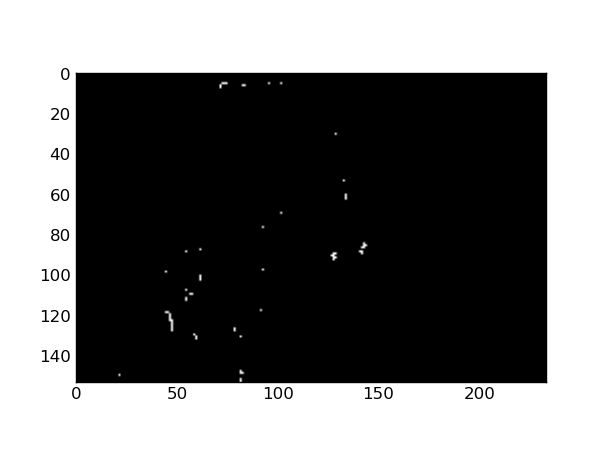
\includegraphics[scale=0.8]{files/premethod/img/houghthreshold.png}
	\caption{Tærskelværdier på houghlinjerne tegnet ud fra sobelbilledets kanter.\label{fig:premethod_houghCellLinesThreshold}}
\end{figure}

Da det er meget svært at evaluere resultatet af dette har vi markeret de tegnede områder på originalbilledet i figur \ref{fig:premethod_houghCellLinesThresholdOnOrig}. Her ses det tydeligt at kun meget få af de røde områder ligger i centrum af en vesikel, mens de fleste ligger langt fra. Som beskrevet i afsnittet om foldning så kan man ikke regne med de yderste pixels i rammen omkring et billede der er blevet foldet. Men selvom man ser bort fra disse virker de røde områder tilfældigt sat i forhold til vesiklerne.

\begin{figure}[H]
	\centering
	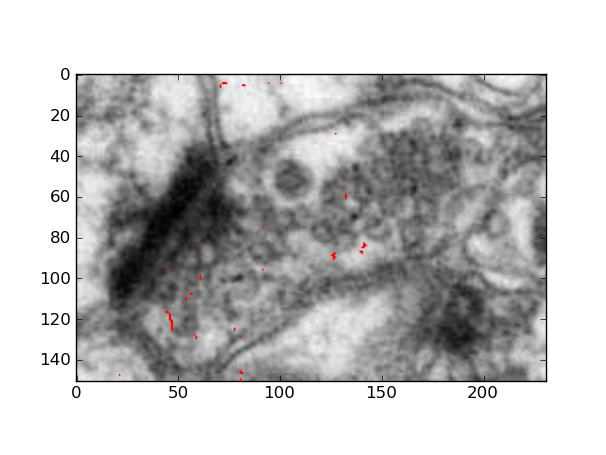
\includegraphics[scale=0.8]{files/premethod/img/houghres.png}
	\caption{De resulterende områder fundet ved hjælp af Hough cirkel detektion plottet på det originale billede.\label{fig:premethod_houghCellLinesThresholdOnOrig}}
\end{figure}


\subsubsection{Afledet Gauss-filter}
Vores resultat af Hough detektionen blev ikke særlig godt. Dette skyldes at billedet som kant detektionen leverer videre indeholder for meget støj, så kanterne ikke fremgår tydelige. En mulig optimering er at benytte et gaussfilter. Et gaussfilter kan benyttes til andet end bare at udglatte billeder. Ved at tage det afledte gaussfilter i hver retning, kan vi lave et nyt filter. Dette filter fremhæver højderygge i billedet, såsom kanterne på en vesikel. Et simpelt eksempel er vist i figur \ref{fig:premethod_gaussCirc} hvor billedet til venstre er originalbilledet af to figurer. I billedet til højre ses så resultatet efter at folde med det nye filter, en flot markeret hvid linje hvor kanten går på begge figurerne.

\begin{figure}[H]
	\begin{minipage}[b]{0.5\linewidth}
		\centering
		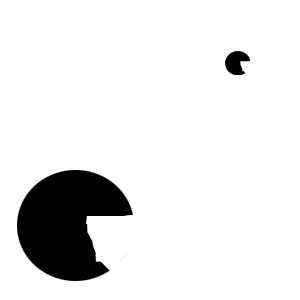
\includegraphics[scale=1.3]{files/premethod/img/gauss_derived_circ1.png}
	\end{minipage}
	\hspace{0.5cm}
	\begin{minipage}[b]{0.5\linewidth}
		\centering
		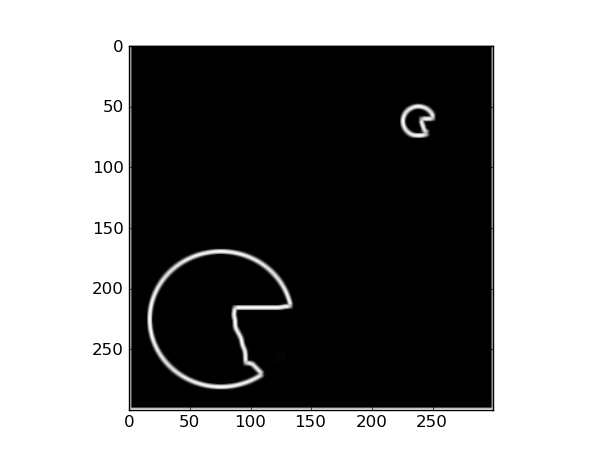
\includegraphics[scale=0.5]{files/premethod/img/gauss_derived_circ2.png}
	\end{minipage}
	\caption{Originalbillede samt det resulterende billede efter foldning med det afledete gaussfilter.\label{fig:premethod_gaussCirc}}
\end{figure}

Dette er et resultat vi meget gerne vil opnå med vores vesikler, da det ønskescenariet vil være at få et bedre af kanterne, der kan benyttes af Hough cirkel detektionen.

Vi har at et gaussfilter i to dimmensioner er lig
\begin{align}
	G(x,y) = \frac{1}{2\pi\sigma^2}e^{-\frac{x^2+y^2}{2\sigma^2}}
\end{align}
og vi har altså at de afledte af gaussfilteret er lig
\begin{align}
	G_x(x,y) = \frac{\partial}{\partial x}G(x,y)=-\frac{x}{2\pi\sigma^4}e^{-\frac{x^2+y^2}{2\sigma^2}} \\
	G_y(x,y) = \frac{\partial}{\partial y}G(x,y)=-\frac{y}{2\pi\sigma^4}e^{-\frac{x^2+y^2}{2\sigma^2}}
\end{align}

Vi finder så vores nye billede ved at folde det originale billede med gaussfilteret afledt i x-retningen, det samme for gassfilteret afledt i y-retningen og så tage kvadratroden af summen af de kvadrerede resultater.
\begin{align}
	I_x = I * G_x && I_y = I * G_y && I_{ny} = \sqrt{I_x^2+I_y^2}
\end{align} 
hvor $I$ er det originale billede, og $G_x$ hhv. $G_y$ er gaussfilteret afledt i x- hhv. y-retningen.

Vi observerer så at som x og y stiger, vil brøken i exponenten gå mod minus uendelig, og exponenten vil altså gå mod 0. Allerede ved $x=y=5$, og en $\sigma$-værdi på 1, vil brøken være lig -25 og $\exp(-25)\sim0$. Denne observation leder os altså til at bygge vores gaussfilter som en 5x5 matrice, da større dimmensioner bare vil have 0 i felterne. Vi flytter så centrum op til (0,0) ved at finde gauss-værdier fra -2 til 2.

Dette giver nedenstående matricer for $G_x$:
\begin{align*}
 &0.00583005  &&0.01306423  &&&0. 			&&&&-0.01306423 &&&&&-0.00583005\\
 &0.02612847  &&0.05854983  &&&0. 			&&&&-0.05854983 &&&&&-0.02612847\\
 &0.04307856  &&0.09653235  &&&0. 			&&&&-0.09653235 &&&&&-0.04307856\\
 &0.02612847  &&0.05854983  &&&0. 			&&&&-0.05854983 &&&&&-0.02612847\\
 &0.00583005  &&0.01306423  &&&0. 			&&&&-0.01306423 &&&&&-0.00583005
\end{align*}
samt $G_y$:
\begin{align*}
	&0.00583005  &&0.02612847  &&&0.04307856  	&&&&0.02612847  &&&&&0.00583005\\
	&0.01306423  &&0.05854983  &&&0.09653235  	&&&&0.05854983  &&&&&0.01306423\\
	&0.          &&0.          &&&0.          	&&&&0.          &&&&&0.        \\
	&-0.01306423 &&-0.05854983 &&&-0.09653235 	&&&&-0.05854983 &&&&&-0.01306423\\
	&-0.00583005 &&-0.02612847 &&&-0.04307856 	&&&&-0.02612847 &&&&&-0.00583005
\end{align*}
og foldet med vores testcellebillede giver det resultatet i figur \ref{fig:premethod_gaussCell}.

\begin{figure}[H]
	\centering
	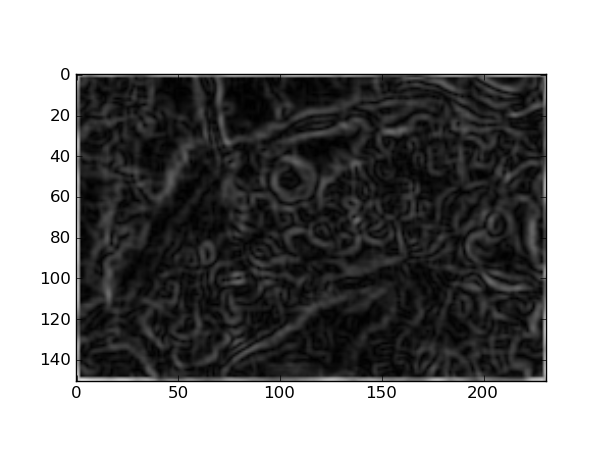
\includegraphics[scale=0.8]{files/premethod/img/gauss_derived_cell2.png}
	\caption{Originalbillede af en celle foldet med det afledete gaussfilter.\label{fig:premethod_gaussCell}}
\end{figure}

Resultatet af dette er ikke hvad vi havde forventet. Der er stadig alt for meget støj omkring vesiklerne og det er ikke blevet nemmere at se hvor de præcis er. Det er samtidig svært at se en synlig forskel i forhold til resultatet med sobelfilteret. Den eneste forskel er at vi her kan styre størrelsen på gausskernen, som f.eks. benyttes i Difference of Gaussians (DoG). Dette giver os ideen til Sum of Derived Gaussians beskrevet i næste afsnit.

\subsubsection{Sum of Derived Gaussians}
Når man folder et billede med et gaussfilter får man et resulterende udglattet billede. Man kan så styre størrelsen på kernen som filteret benytter, hvilket påvirker hvor udglattet billedet bliver. Princippet i Difference of Gaussians (DoG) er at tage to ens gaussfunktioner, kun adskilt af deres kernestørrelse, og trække dem fra hinanden så det giver et nyt filter. Hvis man havde taget det originale billede og foldet med gaussfilteret med en kerne $\sigma_1$ og trukket fra en kopi af det originale billede foldet med gaussfilteret med en kerne $\sigma_2$ så giver det samme resultat som det billedet foldet med DoG filteret. Funktionen viser altså forskellen mellem et billede foldet med gaussfilter med to forskellige kerner. 

Idet vores cellebillede foldet med det afledte gaussfilter, vist i figur \ref{fig:premethod_gaussCell} ovenfor, er lys omkring de steder hvor der er en kant, ved vi at de pixels har værdier større end 0. Vores ide går så ud på at tage forskellige kerner og folde billedet med det afledte gaussfilter. De resulterende billeder skal så i stedet ligges sammen og på dem måde fremhæve de steder der er kanter. Ved at vælge gausskerner der kun fremhæver dele af vesiklerne og ligge sammen med de kerner der viser et tydeligere billede af vesiklerne, er vores håb at vi vil få et bedre kantbillede.

\begin{figure}[H]
	\centering
	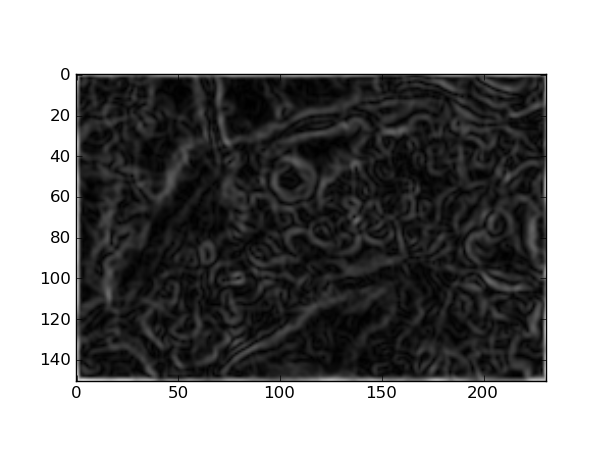
\includegraphics[scale=0.8]{files/premethod/img/sum_der_gauss.png}
	\caption{Originalbillede af en celle foldet med filtret Sum Of Derived Gaussians.\label{fig:premethod_sumOfDiff}}
\end{figure}

I figur \ref{fig:premethod_sumOfDiff} ses det resulterende billede. Det er dog ikke de store ændringer vi kan se i forhold til resultatet før, og vi gør os derfor ikke større forhåbninger for at Hough cirkel detektionen skal finde bedre resultater.

\subsubsection{Foldning med kantkonkur efter vesikelbillede}
Da vi ikke har haft held til at finde vesikelkanter udelukkende ved brug af filtre, vil vi nu i stedet prøve at finde det ved hjælp af en form for matchene billeder. Vores første metode er at tage en generel vesikel og opregne dennes kant. Dette har vi gjort i figur \ref{fig:premethod_vesedge}. 

\begin{figure}[H]
	\centering
	
\includegraphics[scale=0.8]{files/premethod/img/vesikel_edge.png}
	\caption{Vesikel med kantken markeret.\label{fig:premethod_vesedge}}
\end{figure}

I en ny matrice vil vi så indsætte en lav værdi de steder der svarer til kanten på vesiklen, og 0 i resten, som det er vist nedenfor.

\begin{verbatim}
	0,  0,  0,  0,  0,  0,  0,  0,  0,  0,  0,  0,  0,  0,  0,  0,  0 
	0,  0,  0,  0,  0,  0,  0,  0,  0,  0,  0,  0,  0,  0,  0,  0,  0 
	0,  0,  0,  0,  0,  0,  0,  0,  0,  0,  0,  0,  0,  0,  0,  0,  0 
	0,  0,  0,  0,  0,  0,  0,  0,  0,  0,  0,  0,  0,  0,  0,  0,  0 
	0,  0,  0,  0,  0,  0,  0,  0,  0,  0,  0,  0,  0,  0,  0,  0,  0 
	0,  0,  0,  0,  0,-10,-10,-10,-10,-10,-10,  0,  0,  0,  0,  0,  0 
	0,  0,  0,  0,-10,-10,  0,  0,  0,  0,  0,-10,  0,  0,  0,  0,  0 
	0,  0,  0,  0,-10,-10,  0,  0,  0,  0,  0,-10,-10,  0,  0,  0,  0
	0,  0,  0,  0,-10,-10,  0,  0,  0,  0,  0,-10,-10,  0,  0,  0,  0 
	0,  0,  0,  0,-10,-10,  0,  0,  0,  0,  0,  0,  0,-10,  0,  0,  0 
	0,  0,  0,  0,-10,-10,  0,  0,  0,  0,  0,  0,  0,  0,-10,  0,  0 
	0,  0,  0,  0,  0,-10,-10,  0,  0,  0,  0,  0,  0,  0,-10,  0,  0 
	0,  0,  0,  0,  0,  0,-10,  0,  0,  0,  0,  0,  0,-10,  0,  0,  0 
	0,  0,  0,  0,  0,  0,  0,-10,-10,-10,-10,-10,-10,  0,  0,  0,  0 
	0,  0,  0,  0,  0,  0,  0,  0,  0,  0,  0,  0,  0,  0,  0,  0,  0 
	0,  0,  0,  0,  0,  0,  0,  0,  0,  0,  0,  0,  0,  0,  0,  0,  0
\end{verbatim}

Ved at folde denne matrice med vores cellebillede ønsker vi at kanten vil fremstå tydeligt. Vi har prøvet at folde vores cellebillede to gange. Første gang med matricen vist ovenfor, og anden gang med samme matrice, men hvor indgangende inden for hvad der svarer til cellekanten er 10 i stedet for 0. Dette giver billederne i figur \ref{fig:premethod_vesEdgeConv}.

\begin{figure}[H]
	\begin{minipage}[b]{0.5\linewidth}
		\centering
		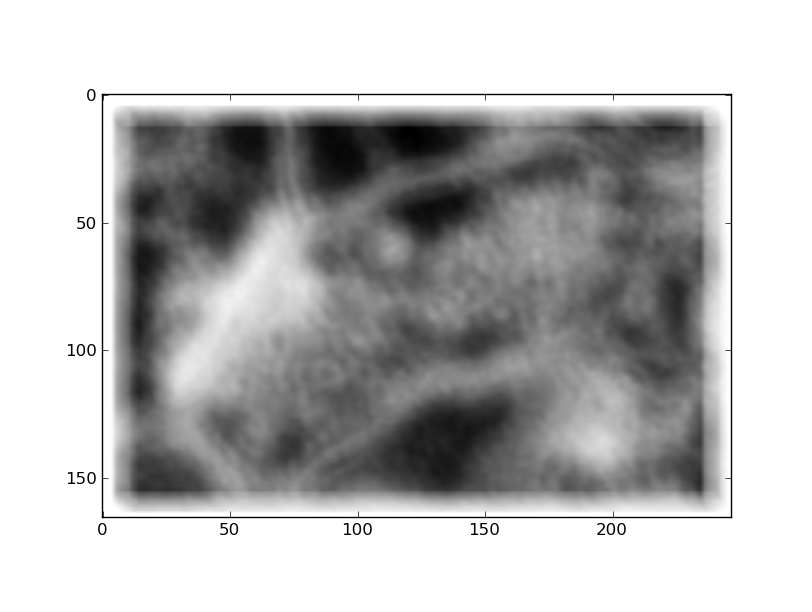
\includegraphics[scale=0.4]{files/premethod/img/convolve_edge1.png}
	\end{minipage}
	\hspace{0.5cm}
	\begin{minipage}[b]{0.5\linewidth}
		\centering
		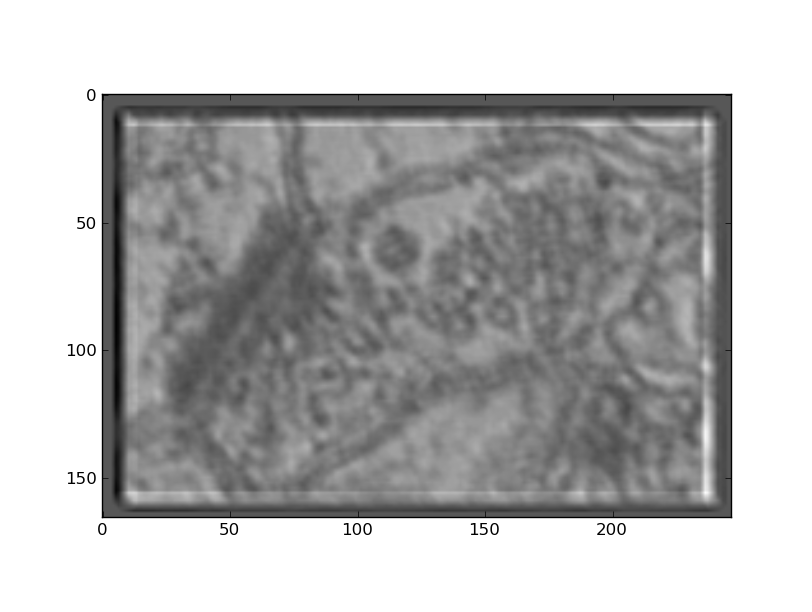
\includegraphics[scale=0.4]{files/premethod/img/convolve_edge2.png}
	\end{minipage}
	\caption{Billeder foldet med matricer. Venstre billede med matrice med 0 i indre. Højre billede med matrice med 10 i indre.\label{fig:premethod_vesEdgeConv}}
\end{figure}

Billederne er meget forskellige, så det er tydeligt at det har en stor betydning med hvilke tal der vælges til hver indgang. I det venstre billede er der svært at se en eneste vesikel, hvorimod den højre er væsentlig tydeligere. Dette resultat er et skridt i den rigtige retning da vi nu begynder at kunne se flere af vesiklerne. Der er dog stadig problemer i venstre side af cellen hvor overgangen mellem vesiklerne er svær at se.

\subsection{Reflektion}
Vi omtalte kort at vesiklerne i figur \ref{fig:premethod_ves1} har forskellige farvet indre. Dette vil vi nu kigge nærmere på. Figur \ref{fig:premethod_vescolors} har indtegnet 3 pile til hver vesikel. Den ene pil peger på vesiklens indre, og de to andre peger på to steder på kanten af vesiklen. 

Tager vi vesiklen til venstre, ses det at der er stor farveforskel på vesiklens indre, og kanten af vesiklen. Det lyseste sted på kanten har stadig en farveværdi på 65 lavere end centrum. En overgang fra kant til centrum er her derfor meget tydelig. Det bemærkes dog også at der er en farveforskel på 33 på det mørkeste og lyseste sted på kanten af vesiklen. 

Tager vi så vesiklen til højre, ser vi at der er en farveforskel på 25 fra det lyseste sted på kanten til det mørkeste. Dette er altså meget det samme som den første vesikel, og farveværdierne ligger da også meget tæt (120 versus 121 for lyseste og 87 versus 96 for det mørkeste). Den store forskel ses når vi tager en pixel fra centrum. Denne har en værdi på 114 (versus 185 i den første) og har altså en farveforskel på kun 7 i forhold til det lyseste sted på kanten.

\begin{figure}[H]
	\centering
	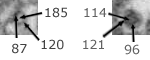
\includegraphics[scale=5]{files/premethod/img/ves_colors.png}
	\caption{Vesikler med 3 farveværdier hver.\label{fig:premethod_vescolors}}
\end{figure}

At der er så stor farveforskel på kanterne er dog ikke den eneste udfordring. Kanterne består ikke af rene linjer uden huller imellem. Zoomer man ind på et billede af en vesikel ses det tydeligt at der er store huller mellem de farvede pixels der udgør kanten. Ligges disse ting sammen med at vesiklerne ligger tæt op ad andre vesikler, samt andet støj, er det klart at almindelige filtre samt kant detektorer ikke kan benyttes til vores problem. 

Det bedste billede vi har fået, er ved at detektere kanten i en vesikel ved hjælp af en matrice bestående af informationer om en generel vesikel. Dette resultat inspirerer os til at lave en funktion der detekterer selve vesiklen, ved hjælp af billeder af den selv, hvilket vi præsenterer i næste afsnit. % REF GOES HERE.

%% Kildeangivelser:
% http://en.wikipedia.org/w/index.php?title=Image_gradient&oldid=421160257
% http://en.wikipedia.org/w/index.php?title=Gaussian_blur&oldid=422700764
% http://en.wikipedia.org/w/index.php?title=Sobel_operator&oldid=422155717
% http://en.wikipedia.org/w/index.php?title=Hough_transform&oldid=422150042
% http://en.wikipedia.org/w/index.php?title=Canny_edge_detector&oldid=421218460
% http://en.wikipedia.org/w/index.php?title=Edge_detection&oldid=425584110
% http://en.wikipedia.org/w/index.php?title=Difference_of_Gaussians&oldid=418426534
